
% JuliaCon proceedings template
\documentclass{juliacon}
\usepackage{tikz}
\usepackage{svg}
\usetikzlibrary{patterns, arrows.meta}

% **************GENERATED FILE, DO NOT EDIT**************

\title{A Fast, Stable Variant on Quicksort}

\author[1]{Lilith Hafner}
\author[1]{Kobina Thatcher}
\affil[1]{Independent Researcher}

\keywords{Julia, Performance, Sorting}



\begin{document}

\maketitle

\begin{abstract}

% A brief summary of the paper, providing an overview of the research problem, methodology, main findings, and conclusions.

% We present a stable, out-of place variant of the QuickSort algorithm; prove its correctness, stability, and asymptotic performance characteristics; and empirically demonstrate that it outperforms conventional, unstable, QuickSort implementations on a variety of sorting tasks and architectures.

We present a QuickSort partitioning method that is stable and faster than existing partitioning methods on modern architectures at the cost of requiring auxiliary memory.

\headingtable

\end{abstract}

See \cite{quicksort} for a description of the QuickSort algorithm and \cite{lomuto} for how it can be extended to support alternative partitioning schemes. This paper assumes a familiarity with both these concepts and does not explain them in detail. A video presentation similar to this paper is available at \href{https://youtu.be/RIhCBTx5TYA}{youtu.be/RIhCBTx5TYA}

\section{Partitioning scheme}

The partitioning algorithm requires a source array containing the data to be partitioned and a destination array of equal size to which the partitioned data will be written. To execute the partition, compare each element of the source array with the pivot. Simultaniously, fill the destination array both from the start and from the end by placing the elements less than the pivot at the beginning of the free space in the destination array and the elements greater than the pivot at the end of the free space in the destination array. In pseudocode,

\begin{lstlisting}
To partition from source to destitantion,
    let start of free space = first index of destination
    and let end of free space = last index of destination
    for each element in source,
        if the element is less than the pivot
            put it at the start of free space
            and increment free space.
        Otherwise,
            put it at the end of free space
            and decrement end of free space.
\end{lstlisting}

After executing this partition, all elements from the source array which are less than the pivot will appear in the same order they originally appeared, but shifted to the start of the destination array. Elements greater than or equal to the pivot will appear at the end of destination array and in reverse order. This complete reversal of one sub-array is much more conducive to restoring stability than the complex mixing created by the Hoare \cite{quicksort} or Lomuto \cite{lomuto} partitioning schemes.

\section{Stability}

Stability is a property of a sorting algorithm that guarantees that any elements which compare equivalently (i.e. neither is less than the other) will appear in the final output in the same order as they appear in the input.

We extend the notion of stability to intermediary results and say that a block of memory is stable if every pair of elements which compare equivalently within that block of memory appear in the same order as they appear in the input. We also define a notion of reverse-stability and say that a block of memory is reverse-stable if every pair of elements that compare equivalently is not in the same order as they appear in the input.

Informally, we model stability as the algorithm progresses like so

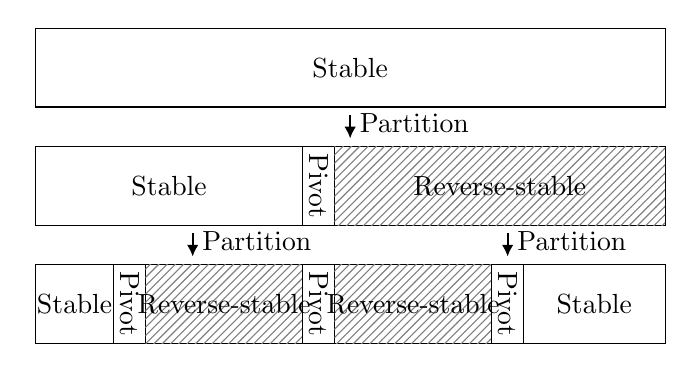
\begin{tikzpicture}
    % First rectangle
    \draw (0,0) rectangle (8,-1);
    \node at (4,-0.5) {Stable};

    \draw[-{Latex[length=1.5mm, width=1.5mm]}, thick] (4,-1.1) -- (4,-1.4);
    \node at (4,-1.2) [right] {Partition};

    % Second rectangle
    \draw (0,-1.5) rectangle (8,-2.5);
    \node at (1.7,-2) {Stable};
    \draw (3.4,-1.5) -- (3.4,-2.5);
    \node[rotate=270] at (3.6,-2) {Pivot};
    \draw (3.8,-1.5) -- (3.8,-2.5);
    \fill[pattern=north east lines, pattern color=gray] (3.8,-1.5) rectangle (8,-2.5);
    \node at (5.9,-2) {Reverse-stable};

    \draw[-{Latex[length=1.5mm, width=1.5mm]}, thick] (2,-2.6) -- (2,-2.9);
    \node at (2,-2.7) [right] {Partition};

    \draw[-{Latex[length=1.5mm, width=1.5mm]}, thick] (6,-2.6) -- (6,-2.9);
    \node at (6,-2.7) [right] {Partition};

    % Third rectangle
    \draw (0,-3) rectangle (8,-4);
    \node at (0.5,-3.5) {Stable};
    \draw (1.0,-3) -- (1.0,-4);
    \node[rotate=270] at (1.2,-3.5) {Pivot};
    \draw (1.4,-3) -- (1.4,-4);
    \fill[pattern=north east lines, pattern color=gray] (1.4,-3) rectangle (3.4,-4);
    \node at (2.4,-3.5) {Reverse-stable};
    \draw (3.4,-3) -- (3.4,-4);
    \node[rotate=270] at (3.6,-3.5) {Pivot};
    \draw (3.8,-3) -- (3.8,-4);
    \fill[pattern=north east lines, pattern color=gray] (3.8,-3) rectangle (5.8,-4);
    \node at (4.8,-3.5) {Reverse-stable};
    \draw (5.8,-3) -- (5.8,-4);
    \node[rotate=270] at (6,-3.5) {Pivot};
    \draw (6.2,-3) -- (6.2,-4);
    \node at (7.1,-3.5) {Stable};
\end{tikzpicture}

Each partition splits the input into a stable sub-array and a reverse-stable sub-array where the first sub-array is of the same stability as the partition's input and the second sub-array is the opposite stability. Further, any pair of equivalent elements separated by a pivot always appear in the same order as they do in the input.

Elements less than and greater than the pivot are already handled correctly by the algorithm presented above. However, elements equal to the pivot must be placed after the pivot iff they occur after the pivot in the input. To do this, we split the partitioning loop in two. First we iterate over the elements before the pivot, branching on weather they are less than or equivalent to the pivot element; and then we iterate over the elements after the pivot, branching on whether they are strictly less than the pivot. Concretely, this may be implemented as

\begin{lstlisting}[language=Julia]
function partition!(destination, source, pivot_index)
    pivot = source[pivot_index]
    destination_start = firstindex(destination)
    destination_end = lastindex(destination)
    for element in @view source[begin:pivot_index-1]
        if element <= pivot # Loose inequality
            destination[destination_start] = element
            destination_start += 1
        else
            destination[destination_end] = element
            destination_end -= 1
        end
    end
    for element in @view source[pivot_index+1:end]
        if element < pivot # Strict inequality
            destination[destination_start] = element
            destination_start += 1
        else
            destination[destination_end] = element
            destination_end -= 1
        end
    end
    @assert destination_start == destination_end
    destination[destination_start] = pivot
end
\end{lstlisting}

In order for the final result to be stable, we may use a stable sorting algorithm as the base case for stable base cases and a reverse-stable sorting algorithm for reverse-stable base cases. Reverse-stable base case sorting algorithms are not the focus of this paper but can easily be formed by reversing the input and then applying a stable sorting algorithm such as insertion sort.

\section{Performance}

\scalebox{.5}{\includesvg{fig.svg}}

\subsection{Reproducibility}

The figure above can be quickly reproduced by installing the Julia package hosted at \href{https://github.com/LilithHafner/QuickerSort.jl}{github.com/LilithHafner/QuickerSort.jl} and running \lstinline{QuickerSort.reproduce_figure().}

\section{Deployment and reference implementations}

The partitioning scheme presented in this paper is, as of the date of publication, used in the default sorting algorithm in the Julia standard library. It was selected because of superior performance over the existing Hoare partitioning method\cite{PR}.

A simplified and optimized version that is not enmeshed with Julia's multiple dispatch-based sorting optimizations is available at \href{https://github.com/LilithHafner/QuickerSort.jl}{https://github.com/LilithHafner/QuickerSort.jl}  and used for the benchmark results above.

\hrule

\section{Old stuff}

\hrule

\section{Introduction}

Sorting features prominently in many areas of computer science and can form a bottleneck in certain data-analysis tasks. Consequently, optimizing the performance of existing algorithms and devising new algorithms with improved properties has a significant impact spread across many domains of applied computer science.

We present a variant on QuickSort\cite{quicksort} that is both stable and is faster than conventional QuickSort, at the cost of requiring a scratch space to operate.

\subsection{Stability}

A sorting algorithm is said to be stable if elements which compare equally are not re-arranged by sorting. For example, if sorting a vector of $(name, age)$ pairs by age, a stable sorting algorithm will stratify the dataset by age while preserving the order of names within a given age. On the other hand, an unstable algorithm may arbitrarily permute entries of a given age. Stable sorting is a strictly harder task than unstable sorting. MergeSort is stable \cite{mergesort}, QuickSort is unstable \cite{quicksort}, AnotherFancyAlgorithm is unstable \cite{another_fancy_algorithm} and ScratchQuickSort is stable. \ref{ref} for proof of ScratchQuickSort's stability space complexity.

\subsection{Auxiliary memory}

TODO: find a paper that defines this concept and adopt their definitions.

An algorithm is said to operate \textit{in place} if it's auxiliary space complexity, i.e. the amount of memory it requires beyond what is required to store its input, is less than $O(n)$. Operating in-place is important when a dataset takes up almost all of a system's available memory in which case a small constant factor increase in space consumption can result in significant slowdowns or prevent an operation from completing altogether. Sorting algorithms have a variety of auxiliary space requirements. For example, MergeSort is not in place, as it uses $\frac{n}{2} + k\log(n) = \Theta(n)$ additional space. QuickSort uses $\Theta(\log(n))$ additional space (to store a stack) and InsertionSort uses $\Theta(1)$ additional space so they are in place. ScratchQuickSort is not in place, because it uses $n + k\log(n) = \Theta(n)$ additional space. See section \ref{ref} for proof of ScratchQuickSort's auxiliary space complexity.

\subsection{Comparison based sorting}

A key aspect of sorting that makes it widely used is that it encapsulates a complicated algorithm in a simple API. This enables application and library developers to utilize state of the art optimizations without any distraction from their domain of expertise. Comparison based sorting algorithms, the object of this paper, require only a comparison function and a mutable array of pairwise comparable objects. A wide variety of sorting optimizations exist which require a more complex API for sorting custom objects, most notably radix sort, but we do not concern ourselves with those optimizations here because of the added burden on sorting users which often outweighs runtime improvements over already very fast algorithms.

\section{Literature Review/Related algorithms}

Engineering of a Quicksort Partitioning Algorithm
  - Alternative partitioning algorithms
  - We could claim that scratch quick sort is a partitioning algorithm... it kinda is, that's the main innovation.
  - This paper's presentation is shit
  - minor refactoring of naive implementation for increased perf? IDK. Maybe use sentinals to avoid bounds checking?

Review on Performance of Quick Sort Algorithm
  - Abstract has typos...
  - Survey paper
  - Meh.
  - "The purpose of this paper is to prove that Multiple Pivot Sort algorithm is better than other sorting algorithm through empirical study."
  - Implements in python and compares runtime empirically... totally invalid methodology

Review on Sorting Algorithms A Comparative Study
  - Compares runtime of merge/quick/seleciton/insertion/etc sorts
  - Does not provide methodology
  - rife with typos
  - poor data visualization

\/ \/ \/ \/ This is the one \/

QuickMergesort: Practically Efficient Constant-Factor Optimal Sorting
Edelkamp, S & Weiss, A - QuickMergesort-Practically Efficient Constant-Factor Optimal Sorting
  - This is the first paper so far that I can't rule out as useless from the abstract alone, good work kobina.
  - "Based on QuickHeapsort [5, 7], Edelkamp and Weiß [9] developed the concept of QuickX-sort and applied it to X = WeakHeapsort [8]" TODO: follow all those citations
  - Introsort and Dual-Pivot Quicksort are SOTA practical implementaitons
  - InSituMergesort
  - Absolutely the bee's knees. Read and re-read this paper and some of those it cites

/\/\/\/\ This is the one /\

Optimizing Complexity of Quick Sort
  - "Quick Sort is considered as the fastest sorting algorithm among all the sorting algorithms."
  - Original QS was 1962
  - Computes pivot as \textit{mean} of extrema of first half and second half and claims nlogn worst case like  a fool. Totally bogus

The Quicksort algorithm
and related topics
  - 120 pages long

NQMSort: A Fast and Efficient Way of Sorting
  -"But any Sorting algorithm either works in quadratic time or only works for shorter array sizes."
  - shit

Enhanced Quicksort Algorithm
  - A terribly inefficient version of counting sort
  - Not quicksort at all

Making a fast unstable sorting algorithm stable
  - Good source on radix sorting and friends, not comparison based
  - Reasonable quality

Nearly-Optimal Mergesorts:
Fast, Practical Sorting Methods That
Optimally Adapt to Existing Runs
  - Adaptive mergesort, good for easy case pre-orderings
  - Reasonable quality

Pattern-defeating Quicksort
  - Title says it all
  - Reasonable paper
  - Competative implementaion
  - Good model

Performance Comparison of Sequential Quick Sort and
Parallel Quick Sort Algorithms
  - Paralellization performance

Increasing the efficiency of Quicksort
  - 1970
  - Introduces dual pivot quicksort?

Williams, JWJ - Heapsort
  - 1963
  - Heap (not heapsort)

Sedgewick, R - Implementing Quicksort Programs
  - Practical tips for QuickSort
    - Roll your own stack
    - Recurse on small half
    - Insertionsort all at once
    - Median of 3 partitioning

---

QuickSort
TimSort
PagedMergeSort

\section{Description of the Algorithm}

We call our variant of QuickSort ScratchQuickSort to signify its reliance on a scratch space. It is structured quite similarly to conventional QuickSort, with a custom partitioning method. After selecting a pivot, each element of the sub-array being partitioned is compared to the pivot and then either placed at the beginning or end of the available scratch-space. After this process, the scratch space contains a partitioned copy of the data and we can perform the next iteration of the algorithm copying back from the scratch space to the original array.

We provide a pseudocode implementation here,

\begin{lstlisting}
function scratch_quick_sort(array)
    allocate a scratch space of the same size as array
    call scratch_quick_sort(array, scratch_space, array)
    free the scratch space
end

function scratch_quick_sort(source, target, original_array)
    assert that source and target have the same length
    if the source and target are small
        sort the source using a base case algorithm
        copy source to original_array
    else
        select a pivot element from source
        partition from source to target
        form sub-arrays out of the low values and high values
        swap source and target
        recurse on the smaller sub-array
        recurse on the larger sub-array
    end
end

function partition(source, target, pivot)
    low_pointer = firstindex(target)
    high_pointer = lastindex(target)
    for each element in source
        if that element is less than pivot
            put that element at low_pointer
            increment low_pointer
        else
            put that element at high_pointer
            decrement high_pointer
        end
    end
    return the index that divides low values from high values
end
\end{lstlisting}


\section{Proofs}

\subsection{Asymptotic performance}

\subsection{correctness and stability}

\section{Empirical performance data}

\section{Adoption and deployment}

\section{Role in an in-place sorting algorithm}

All algorithms require at least $O(1)$ auxiliary memory. This memory can be used as a scratch space for ScratchQuickSort, provided the length of inputs provided to ScratchQuickSort is bounded. This enables the use of ScratchQuickSort as a base case for stable, in-place, recursive divide and conquer sorting algorithms such as PagedMergeSort \ref{https://github.com/JuliaCollections/SortingAlgorithms.jl/pull/71}.

For a more modest reduction in auxiliary memory usage, it is possible to perform ScratchQuickSort to sort the first and second half of a vector separately and then merge the results, with all operations using the same scratch space of size $n/2$.

\section{References}

\appendix

\section{Simple Julia implementation}

\section{Optimized Julia implementation}

An optimized implementation in Julia

\begin{lstlisting}
const THRESHOLD = 20

"Use insertion sort to sort `src[lo:hi]` into `dst[lo:hi]`. Stable if rev=false, otherwise reverse-stable."
function smallsort_to!(dst::AbstractVector, src::AbstractVector, lo::Int, hi::Int, rev::Bool)
    @inbounds for i = lo:hi
        j = i
        x = src[i]
        while j > lo
            y = dst[j-1]
            (rev ? !isless(y, x) : isless(x, y)) || break
            dst[j] = y
            j -= 1
        end
        dst[j] = x
    end
end

make_scratch(v::AbstractVector) = similar(v), Memory{Tuple{Int, Int, typeof(v), typeof(v), Bool}}(undef, max(0, Base.top_set_bit(length(v))-Base.top_set_bit(THRESHOLD)))
function quicker_sort!(v::AbstractVector, (t,stack) = make_scratch(v))
    stack_size = 0

    lo, hi = firstindex(v), lastindex(v)

    src = v
    dst = t
    rev = false

    @inbounds if hi - lo > THRESHOLD
        while true

            # src[lo:hi] => dst[lo:hi]

            pivot_index = mod(hash(lo), lo:hi)

            pivot = src[pivot_index]

            large_values = 0

            for i in lo:pivot_index-1
                x = src[i]
                fx = rev ? !isless(x, pivot) : isless(pivot, x)
                dst[(fx ? hi : i) - large_values] = x
                large_values += fx
            end
            for i in pivot_index+1:hi
                x = src[i]
                fx = rev ? isless(pivot, x) : !isless(x, pivot)
                dst[(fx ? hi : i-1) - large_values] = x
                large_values += fx
            end

            new_pivot_index = hi-large_values

            if new_pivot_index-lo < THRESHOLD && hi-new_pivot_index < THRESHOLD
                smallsort_to!(v, dst, lo, new_pivot_index-1, rev)
                smallsort_to!(v, dst, new_pivot_index+1, hi, !rev)
                stack_size == 0 && (v[new_pivot_index] = pivot; break)
                lo, hi, src, dst, rev = stack[stack_size]
                stack_size -= 1
            elseif new_pivot_index-lo < THRESHOLD
                smallsort_to!(v, dst, lo, new_pivot_index-1, rev)
                lo = new_pivot_index+1
                rev = !rev
            elseif hi-new_pivot_index < THRESHOLD
                smallsort_to!(v, dst, new_pivot_index+1, hi, !rev)
                hi = new_pivot_index-1
            elseif new_pivot_index-lo < hi-new_pivot_index
                stack[stack_size += 1] = (new_pivot_index+1, hi, src, dst, !rev)
                hi = new_pivot_index-1
            else
                stack[stack_size += 1] = (lo, new_pivot_index-1, src, dst, rev)
                lo = new_pivot_index+1
                rev = !rev
            end
            dst,src = src,dst

            v[new_pivot_index] = pivot
        end
    else
        smallsort_to!(v, v, lo, hi, false)
    end

    v
end
\end{lstlisting}

\hrule

 computer science research paper typically consists of several sections, which are essential for presenting the research findings and results. Here are the common sections found in a computer science research paper:

    Abstract: A brief summary of the paper, providing an overview of the research problem, methodology, main findings, and conclusions.
    Introduction: An introduction to the research topic, including background information, motivation, and research questions or hypotheses.
    Literature Review: A review of existing research in the field, discussing relevant theories, models, and findings that relate to the research problem.
    Methodology: A description of the research design, methods, and procedures used to collect and analyze data.
    Results: Presentation of the research findings, including data, statistics, and visualizations.
    Discussion: An interpretation of the results, discussing the implications, limitations, and potential applications of the research.
    Conclusion: A summary of the main findings, highlighting the contributions of the research and suggesting avenues for future research.
    References: A list of sources cited in the paper, formatted according to the chosen citation style.
    Appendices: Supplementary materials that support the research, such as additional data, code, or detailed descriptions of methods.

Some papers may also include additional sections, such as:

    Background: A detailed description of the research context, including relevant technical details and background information.
    Related Work: A discussion of previous research related to the current study, highlighting similarities and differences.
    Experimental Design: A detailed description of the experimental design, including the experimental setup, data collection procedures, and data analysis methods.
    Evaluation: An evaluation of the research, discussing the strengths and limitations of the study.
    Future Work: Suggestions for future research directions and potential applications of the research.

Note that the specific sections and their order may vary depending on the research field, journal, or conference.

\hline

\section{Introduction}

The \LaTeX{} document preparation system is a special version of the
\TeX; typesetting program where-in a collection of \TeX; commands
are added to \LaTeX{} to simplify typesetting. Importantly, it allows
the author to concentrate on the logical structure of the document
rather than its visual layout.\vskip 6pt
Moreover, \LaTeX{} provides a consistent and comprehensive document
preparation interface. There are simple-to-use commands for
generating a table of contents, lists of figures and/or tables, and indexes.
\LaTeX{} can automatically number list entries, equations, figures,
tables, and footnotes, as well as articles, sections, and subsections.
Using this numbering system, bibliographic citations, page
references, and cross references to any other numbered entity (e.g.
article, section, equation, figure, list entry, etc.) become quite simple
and straightforward. The use of \LaTeX{} document classes allows
a simple change of class to transform the appearance of your document.\vskip 6pt
\LaTeX{} is a powerful tool for managing long and complex documents.
In particular, partial processing enables long documents to
be produced article by article without losing sequential information.
The use of document classes allows a simple change of style
(or style option) to transform the appearance of your document.



\section{The JuliaCon Article Class}
\label{sec:documentclass}
%
The juliacon class file preserves the standard LATEX{} interface such
that any document that can be produced using the standard LATEX{}
article class can also be produced with the class file.\vskip 6pt
It is likely that the make up will change after file submission. For
this reason, we ask you to ignore details such as slightly long lines,
page stretching, or figures falling out of synchronization, as these
details can be dealt with at a later stage.\vskip 6pt
Use should be made of symbolic references (\verb \ref ) in order to
protect against late changes of order, etc.

\section{USING THE JuliaCon Article CLASS FILE}

If the file \verb juliacon.cls  is not already in the appropriate system directory
for \LaTeX{} files, either arrange for it to be put there or copy
it to your working directory. The \verb juliacon  document class is implemented
as a complete class, not a document style option. In order to
use the \verb juliacon  document class, replace \verb article  by \verb juliacon  in the
\verb \documentclass  command at the beginning of your document:
\vskip 6pt
\begin{centering}
    \verb \documentclass{article}  \end{centering}
\vskip 6pt
replace by
\vskip 6pt
 \verb \documentclass{juliacon}  \vskip 6pt
In general, the following standard document \verb style  options should
{ \itshape not} be used with the {\footnotesize \itshape article} class file:
\begin{enumerate}
\item[(1)] \verb 10pt,  \verb 11pt,  \verb 12pt   ? unavailable;
\item[(2)] \verb twoside  (no associated style file) ? \verb twoside  is the default;
\item[(3)] \verb fleqn, \verb leqno, \verb titlepage ? should not be used;
\end{enumerate}

\section{Additional Document Style Options}
\label{sec:additional_doc}
%
The following additional style option is available with the \verb juliacon  class file:
\vskip 6pt
Please place any additional command definitions at the very start of
the \LaTeX{} file, before the \verb \begin{document} . For example, user-defined
\verb \def  and \verb \newcommand   commands that define macros for
technical expressions should be placed here. Other author-defined
macros should be kept to a minimum.
\vskip 6pt
Commands that differ from the standard \LaTeX{} interface, or that
are provided in addition to the standard interface, are explained in
this guide. This guide is not a substitute for the \LaTeX{} manual itself.
Authors planning to submit their papers in \LaTeX{} are advised to use
\verb \juliacon.cls  as early as possible in the creation of their files.

%
%
%
%
\begin{table*}[t]
\tabcolsep22pt
\tbl{If necessary, the tables can be extended both columns.}{
\begin{tabular}{|l|l|c|c|}\hline
Label & \multicolumn{1}{c|}{Description}
& Number of Users &
Number of Queries\\\hline
Test 1 & Training Data &
\smash{\raise-7pt\hbox{70}} & 104\\
\cline{1-2}\cline{4-4}
Test 2 & Testing Data I & & 105\\\hline
Test 3 & Testing Data II & 30 & 119\\\hline
& Total & 100 & 328\\\hline
\end{tabular}}
\label{tab:symbols}
\begin{tabnote}
This is an example of table footnote.
\end{tabnote}
\end{table*}
% \begin{figure*}[t]
% \centerline{\includegraphics[width=11cm]{juliagraphs.png}}
% \caption{If necessary, the images can be extended both columns.}
%   \label{fig:sample_image}
% \end{figure*}

\section{Additional features}
\label{sec:additional_faci}
In addition to all the standard \LaTeX{} design elements, the \verb juliacon  class file includes the following features:
In general, once you have used the additional \verb juliacon.cls facilities
in your document, do not process it with a standard \LaTeX{} class
file.

\subsection{Titles, Author's Name, and Affiliation}
\label{subsub:title_auth}
The title of the article, author's name, and affiliation are used at the
beginning of the article (for the main title). These can be produced
using the following code:

\begin{verbatim}
\title{ This is an example of article title} }
\author{
   \large 1st Author \\[-3pt]
   \normalsize 1st author's affiliation  \\[-3pt]
    \normalsize 1st line of address \\[-3pt]
    \normalsize 2nd line of address \\[-3pt]
    \normalsize	1st author's email address \\[-3pt]
  \and
   \large 2nd Author \\[-3pt]
   \normalsize 2nd author's affiliation  \\[-3pt]
    \normalsize 1st line of address \\[-3pt]
    \normalsize 2nd line of address \\[-3pt]
    \normalsize	2nd author's email address \\[-3pt]
\and
   \large 3rd Author \\[-3pt]
   \normalsize 3rd author's affiliation  \\[-3pt]
    \normalsize 1st line of address \\[-3pt]
    \normalsize 2nd line of address \\[-3pt]
    \normalsize	3rd author's email address \\[-3pt]
}
\maketitle
\end{verbatim}

\subsection{Writing Julia code}

A special environment is already defined for Julia code,
built on top of \textit{listings} and \textit{jlcode}.

\begin{verbatim}
\begin{lstlisting}[language = Julia]
using Plots

x = -3.0:0.01:3.0
y = rand(length(x))
plot(x, y)
\end{lstlisting}
\end{verbatim}
\begin{lstlisting}[language = Julia]
using Plots

x = -3.0:0.01:3.0
y = rand(length(x))
plot(x, y)
\end{lstlisting}


\subsection{Abstracts, Key words, term etc...}
\label{subsub:abs_key_etc}

At the beginning of your article, the title should be generated
in the usual way using the \verb \maketitle  command. For general terms and keywords use
\verb \terms ,
\verb \keywords  commands respectively. The abstract should be enclosed
within an abstract environment, All these environment
can be produced using the following code:
\begin{verbatim}
\terms{Experimentation, Human Factors}

\keywords{Face animation, image-based modelling...}

\begin{abstract}
In this paper, we propose a new method for the
systematic determination of the model's base of
time varying delay system. This method based on
the construction of the classification data related
to the considered system. The number, the orders,
the time delay and the parameters of the local
models are generated automatically without any
knowledge about the full operating range of the
process. The parametric identification of the local
models is realized by a new recursive algorithm for
on line identification of systems with unknown time
delay. The proposed algorithm allows simultaneous
estimation of time delay and parameters of
discrete-time systems. The effectiveness of
the new method has been illustrated through
simulation.
\end{abstract}

\end{verbatim}

\section{Some guidelines}
\label{sec:some_guide}
The following notes may help you achieve the best effects with the
\verb juliacon  class file.

\subsection{Sections}
\label{subsub:sections}
\LaTeXe{}  provides four levels of section headings and they are all
defined in the \verb juliacon  class file:
\begin{itemize}
\item \verb \section   \item \verb \subsection  \item \verb \subsubsection  \item \verb \paragraph  \end{itemize}
Section headings are automatically converted to allcaps style.
\subsection{Lists}
\label{sec:lists}
%
The \verb juliacon   class file provides unnumbered lists using the
\verb unnumlist  environment for example,

\begin{unnumlist}
\item First unnumbered item which has no label and is indented from the
left margin.
\item Second unnumbered item.
\item Third unnumbered item.
\end{unnumlist}
The unnumbered list which has no label and is indented from the
left margin. was produced by:
\begin{verbatim}
\begin{unnumlist}
\item First unnumbered item...
\item Second unnumbered item...
\item Third unnumbered item...
\end{unnumlist}
\end{verbatim}

The \verb juliacon   class file also provides hyphen list using the
\verb itemize  environment for example,
\begin{itemize}
\item First unnumbered bulleted item which has no label and is indented
from the left margin.
\item Second unnumbered bulleted item.
\item Third unnumbered bulleted item which has no label and is indented
from the left margin.
\end{itemize}
was produced by:
\begin{verbatim}
\begin{itemize}
\item First item...
\item Second item...
\item Third item...
\end{itemize}
\end{verbatim}

Numbered list is also provided in acmtog class file using the
enumerate environment for example,
\begin{enumerate}
\item The attenuated and diluted stellar radiation.
\item Scattered radiation, and
\item Reradiation from other grains.
\end{enumerate}

was produced by:
\begin{verbatim}
\begin{enumerate}
\item The attenuated...
\item Scattered radiation, and...
\item Reradiation from other grains...
\end{enumerate}
\end{verbatim}
\subsection{Illustrations (or figures)}
\label{subsub:sec_Illus}
The \verb juliacon   class file will cope with most of the positioning of
your illustrations and you should not normally use the optional positional
qualifiers on the \verb figure   environment that would override
these decisions.
\vskip 6pt

%
\begin{figure}[t]
\centerline{\includegraphics[width=4cm]{juliagraphs.png}}
\caption{This is example of the image in a column.}
	\label{fig:sample_figure}
\end{figure}

The figure \ref{fig:sample_figure} is taken from the JuliaGraphs
organization \footnote{https://github.com/JuliaGraphs}.

Figure captions should be \emph{below} the figure itself, therefore the
\verb \caption  command should appear after the figure or space left for
an illustration. For example, Figure 1 is produced using the following
commands:

\begin{verbatim}
\begin{figure}
\centerline{\includegraphics[width=20pc]{Graphics.eps}}
\caption{An example of the testing process for a
binary tree. The globa null hypothesis is tested
first at level $\alpha$ (a), and the level of
individual variables is reached last (d). Note
that individual hypotheses can be tested at
level $\alpha/4$ and not $\alpha/8$ as one might
expect at first.}
\label{sample-figure_2}
\end{figure}
\end{verbatim}
Figures can be resized using first and second argument of
\verb \includegraphics   command. First argument is used for modifying
figure height and the second argument is used for modifying
figure width respectively.
\vskip 6pt
Cross-referencing of figures, tables, and numbered, displayed
equations using the \verb \label  and \verb \ref   commands is encouraged.
For example, in referencing Figure 1 above, we used
\verb Figure~\ref{sample-figure}   \subsection{Tables}
\label{subsub:sec_Tab}
The \verb juliacon   class file will cope with most of the positioning of
your tables and you should not normally use the optional positional qualifiers on the table environment which would override these
decisions. Table captions should be at the top.
\begin{verbatim}
\begin{table}
\tbl{Tuning Set and Testing Set}{
\begin{tabular}{|l|l|c|c|}\hline
Label & \multicolumn{1}{c|}{Description}
& Number of Users &
Number of Queries\\\hline
Train70 & Training Data &
\smash{\raise-7pt\hbox{70}} & 104\\
\cline{1-2}\cline{4-4}
Test70 & Testing Data I & & 105\\\hline
Test30 & Testing Data II & 30 & 119\\\hline
& Total & 100 & 328\\\hline
\end{tabular}}
\end{table}\end{verbatim}

\begin{table}
\tbl{Tuning Set and Testing Set}{
\begin{tabular}{|l|l|c|c|}\hline
Label & \multicolumn{1}{c|}{Description}
& Number of Users &
Number of Queries\\\hline
Test 1 & Training Data &
\smash{\raise-7pt\hbox{70}} & 104\\
\cline{1-2}\cline{4-4}
Test 2 & Testing Data I & & 105\\\hline
Test 3 & Testing Data II & 30 & 119\\\hline
& Total & 100 & 328\\\hline
\end{tabular}}
\end{table}
\subsection{Landscaping Pages}
\label{subsub:landscaping_pages}
If a table is too wide to fit the standard measure, it may be turned,
with its caption, to 90 degrees. Landscape tables cannot be produced
directly using the \verb juliacon   class file because \TeX{} itself cannot
turn the page, and not all device drivers provide such a facility.
The following procedure can be used to produce such pages.
\vskip 6pt
Use the package \verb rotating   in your document and change the coding
from
\begin{verbatim}
\begin{table}...\end{table}
to
\begin{sidewaystable}...\end{sidewaystable}
and for figures
\begin{figure}...\end{figure}
to
\begin{sidewaysfigure}...\end{sidewaysfigure}
\end{verbatim}

environments in your document to turn your table on the appropriate
page of your document. For instance, the following code prints
a page with the running head, a message half way down and the
table number towards the bottom.
\begin{verbatim}
\begin{sidewaystable}
\tbl{Landscape table caption to go here.}{...}
\label{landtab}
\end{sidewaystable}
\end{verbatim}

\subsection{Double Column Figure and Tables}
\label{subsub:double_fig_tab}
For generating the output of figures and tables in double column
we can use the following coding:

\begin{enumerate}
\item For Figures:
\begin{verbatim}
\begin{figure*}...\end{figure*}
\end{verbatim}
\item For landscape figures:
\begin{verbatim}
\begin{sidewaysfigure*}...\end{sidewaysfigure*}
\end{verbatim}
\item For Tables:
\begin{verbatim}
\begin{table*}...\end{table*}
\end{verbatim}
\item For landscape tables:
\begin{verbatim}
\begin{sidewaystable*}...\end{sidewaystable*}
\end{verbatim}
\end{enumerate}

\subsection{Typesetting Mathematics}
\label{subsub:type_math}
The \verb juliacon class file will set displayed mathematics with center to
the column width, provided that you use the \LaTeXe{} standard of
open and closed square brackets as delimiters.
The equation
\[
\sum_{i=1}^p \lambda_i = (S)
\]

was typeset using the acmtog class file with the commands

\begin{verbatim}
\[
\sum_{i=1}^p \lambda_i = (S)
\]
\end{verbatim}

For display equations, cross-referencing is encouraged. For example,
\begin{verbatim}
\begin{equation}
(n-1)^{-1} \sum^n_{i=1} (X_i - \overline{X})^2.
\label{eq:samplevar}
\end{equation}
Equation~(\ref{eq:samplevar}) gives the formula for
sample variance.
\end{verbatim}
The following output is generated with the above coding:
\begin{equation}
(n-1)^{-1} \sum^n_{i=1} (X_i - \overline{X})^2.
\label{eq:samplevar}
\end{equation}
Equation~(\ref{eq:samplevar}) gives the formula for
sample variance.


\subsection{Enunciations}
\label{subsub:enunciation}
The \verb juliacon   class file generates the enunciations with the help of
the following commands:
\begin{verbatim}
\begin{theorem}...\end{theorem}
\begin{strategy}...\end{strategy}
\begin{property}...\end{property}
\begin{proposition}...\end{proposition}
\begin{lemma}...\end{lemma}
\begin{example}...\end{example}
\begin{proof}...\end{proof}
\begin{definition}...\end{definition}
\begin{algorithm}...\end{algorithm}
\begin{remark}...\end{remark}
\end{verbatim}
The above-mentioned coding can also include optional arguments
such as
\begin{verbatim}
\begin{theorem}[...]. Example for theorem:
\begin{theorem}[Generalized Poincare Conjecture]
Four score and seven ... created equal.
\end{theorem}
\end{verbatim}

\begin{theorem}[Generalized Poincare Conjecture]
Four score and seven years ago our fathers brought forth,
upon this continent, a new nation, conceived in Liberty,
 and dedicated to the proposition that all men are
created equal.
\end{theorem}


\subsection{Extract}
\label{subsub:extract}
Extract environment should be coded within
\begin{verbatim}
\begin{extract}..\end{extract}
\end{verbatim}

\subsection{Balancing column at last page}
\label{subsub:Balance}
For balancing the both column length at last page use :
\begin{verbatim}
\vadjust{\vfill\pagebreak}
\end{verbatim}

%\vadjust{\vfill\pagebreak}

at appropriate place in your \TeX{} file or in bibliography file.

\section{Handling references}
\label{subsub:references}
References are most easily (and correctly) generated using the
BIBTEX, which is easily invoked via
\begin{verbatim}
\bibliographystyle{juliacon}
\bibliography{ref}
\end{verbatim}
When submitting the document source (.tex) file to external
parties, the ref.bib file should be sent with it.
\cite{bezanson2017julia}

\input{bib.tex}

\end{document}

% Inspired by the International Journal of Computer Applications template
